\documentclass[journal,12pt,twocolumn]{IEEEtran}
%
\usepackage{setspace}
\usepackage{gensymb}
\usepackage{siunitx}
\usepackage{tkz-euclide} 
\usepackage{textcomp}
\usepackage{standalone}
\usetikzlibrary{calc}
\newcommand\hmmax{0}
\newcommand\bmmax{0}

%\doublespacing
\singlespacing

%\usepackage{graphicx}
%\usepackage{amssymb}
%\usepackage{relsize}
\usepackage[cmex10]{amsmath}
%\usepackage{amsthm}
%\interdisplaylinepenalty=2500
%\savesymbol{iint}
%\usepackage{txfonts}
%\restoresymbol{TXF}{iint}
%\usepackage{wasysym}
\usepackage{amsthm}
%\usepackage{iithtlc}
\usepackage{mathrsfs}
\usepackage{txfonts}
\usepackage{stfloats}
\usepackage{bm}
\usepackage{cite}
\usepackage{cases}
\usepackage{subfig}
%\usepackage{xtab}
\usepackage{longtable}
\usepackage{multirow}
%\usepackage{algorithm}
%\usepackage{algpseudocode}
\usepackage{enumitem}
\usepackage{mathtools}
\usepackage{steinmetz}
\usepackage{tikz}
\usepackage{circuitikz}
\usepackage{verbatim}
\usepackage{tfrupee}
\usepackage[breaklinks=true]{hyperref}
%\usepackage{stmaryrd}
\usepackage{tkz-euclide} % loads  TikZ and tkz-base
%\usetkzobj{all}
\usetikzlibrary{calc,math}
\usepackage{listings}
    \usepackage{color}                                            %%
    \usepackage{array}                                            %%
    \usepackage{longtable}                                        %%
    \usepackage{calc}                                             %%
    \usepackage{multirow}                                         %%
    \usepackage{hhline}                                           %%
    \usepackage{ifthen}                                           %%
  %optionally (for landscape tables embedded in another document): %%
    \usepackage{lscape}     
\usepackage{multicol}
\usepackage{chngcntr}
\usepackage{amsmath}
\usepackage{cleveref}
\usepackage{amsmath}
%\usepackage{enumerate}

%\usepackage{wasysym}
%\newcounter{MYtempeqncnt}
\DeclareMathOperator*{\Res}{Res}
%\renewcommand{\baselinestretch}{2}
\renewcommand\thesection{\arabic{section}}
\renewcommand\thesubsection{\thesection.\arabic{subsection}}
\renewcommand\thesubsubsection{\thesubsection.\arabic{subsubsection}}

\renewcommand\thesectiondis{\arabic{section}}
\renewcommand\thesubsectiondis{\thesectiondis.\arabic{subsection}}
\renewcommand\thesubsubsectiondis{\thesubsectiondis.\arabic{subsubsection}}

% correct bad hyphenation here
\hyphenation{op-tical net-works semi-conduc-tor}
\def\inputGnumericTable{}                                 %%

\lstset{
%language=C,
frame=single, 
breaklines=true,
columns=fullflexible
}
%\lstset{
%language=tex,
%frame=single, 
%breaklines=true
%}
\usepackage{graphicx}
\usepackage{pgfplots}

\begin{document}


\newtheorem{theorem}{Theorem}[section]
\newtheorem{problem}{Problem}
\newtheorem{proposition}{Proposition}[section]
\newtheorem{lemma}{Lemma}[section]
\newtheorem{corollary}[theorem]{Corollary}
\newtheorem{example}{Example}[section]
\newtheorem{definition}[problem]{Definition}
%\newtheorem{thm}{Theorem}[section] 
%\newtheorem{defn}[thm]{Definition}
%\newtheorem{algorithm}{Algorithm}[section]
%\newtheorem{cor}{Corollary}
\newcommand{\BEQA}{\begin{eqnarray}}
\newcommand{\EEQA}{\end{eqnarray}}
\newcommand{\define}{\stackrel{\triangle}{=}}
\bibliographystyle{IEEEtran}
%\bibliographystyle{ieeetr}
\providecommand{\mbf}{\mathbf}
\providecommand{\abs}[1]{\ensuremath{\left\vert#1\right\vert}}
\providecommand{\norm}[1]{\ensuremath{\left\lVert#1\right\rVert}}
\providecommand{\mean}[1]{\ensuremath{E\left[ #1 \right]}}
\providecommand{\pr}[1]{\ensuremath{\Pr\left(#1\right)}}
\providecommand{\qfunc}[1]{\ensuremath{Q\left(#1\right)}}
\providecommand{\sbrak}[1]{\ensuremath{{}\left[#1\right]}}
\providecommand{\lsbrak}[1]{\ensuremath{{}\left[#1\right.}}
\providecommand{\rsbrak}[1]{\ensuremath{{}\left.#1\right]}}
\providecommand{\brak}[1]{\ensuremath{\left(#1\right)}}
\providecommand{\lbrak}[1]{\ensuremath{\left(#1\right.}}
\providecommand{\rbrak}[1]{\ensuremath{\left.#1\right)}}
\providecommand{\cbrak}[1]{\ensuremath{\left\{#1\right\}}}
\providecommand{\lcbrak}[1]{\ensuremath{\left\{#1\right.}}
\providecommand{\rcbrak}[1]{\ensuremath{\left.#1\right\}}}
\theoremstyle{remark}
\newtheorem{rem}{Remark}
\newcommand{\sgn}{\mathop{\mathrm{sgn}}}
\providecommand{\res}[1]{\Res\displaylimits_{#1}} 
%\providecommand{\norm}[1]{\lVert#1\rVert}
\providecommand{\mtx}[1]{\mathbf{#1}}
\providecommand{\fourier}{\overset{\mathcal{F}}{ \rightleftharpoons}}
%\providecommand{\hilbert}{\overset{\mathcal{H}}{ \rightleftharpoons}}
\providecommand{\system}{\overset{\mathcal{H}}{ \longleftrightarrow}}
	%\newcommand{\solution}[2]{\textbf{Solution:}{#1}}
\newcommand{\solution}{\noindent \textbf{Solution: }}
\newcommand{\cosec}{\,\text{cosec}\,}
\providecommand{\dec}[2]{\ensuremath{\overset{#1}{\underset{#2}{\gtrless}}}}
\newcommand{\myvec}[1]{\ensuremath{\begin{pmatrix}#1\end{pmatrix}}}
\newcommand{\mydet}[1]{\ensuremath{\begin{vmatrix}#1\end{vmatrix}}}
%\numberwithin{equation}{section}
\numberwithin{equation}{subsection}
%\numberwithin{problem}{section}
%\numberwithin{definition}{section}
\makeatletter
\@addtoreset{figure}{problem}
\makeatother
\let\StandardTheFigure\thefigure
\let\vec\mathbf
%\renewcommand{\thefigure}{\theproblem.\arabic{figure}}
\renewcommand{\thefigure}{\theproblem}
%\setlist[enumerate,1]{before=\renewcommand\theequation{\theenumi.\arabic{equation}}
%\counterwithin{equation}{enumi}
%\renewcommand{\theequation}{\arabic{subsection}.\arabic{equation}}
\def\putbox#1#2#3{\makebox[0in][l]{\makebox[#1][l]{}\raisebox{\baselineskip}[0in][0in]{\raisebox{#2}[0in][0in]{#3}}}}
     \def\rightbox#1{\makebox[0in][r]{#1}}
     \def\centbox#1{\makebox[0in]{#1}}
     \def\topbox#1{\raisebox{-\baselineskip}[0in][0in]{#1}}
\vspace{3cm}
\title{Polynomial Curve Fitting}
\maketitle
\newpage
%\tableofcontents
\bigskip
\renewcommand{\thefigure}{\theenumi}
\renewcommand{\thetable}{\theenumi}
\begin{abstract}
This document contains theory involved in curve fitting.
\end{abstract}
\section{\textbf{Objective}}
The objective is to fit best line for the polynomial curve using regularization.
\section{Generate Dataset}
Create a sinusoidal function of the form
\begin{align}
    y = A\sin{2\pi x} + n(t) \label{eq:1}
\end{align}
n(t) is the random noise that is included in the training set. This set consists of N samples of input data i.e. x expressed as shown below
\begin{align}
    x = \myvec{x_{1}, x_{2}, .., x_{N}}^{T}
\end{align}
which give the corresponding values of y denoted as
\begin{align}
    y = \myvec{y_{1}, y_{2}, .., y_{N}}^{T}
\end{align}
\begin{figure}[!h]
\begin{center}
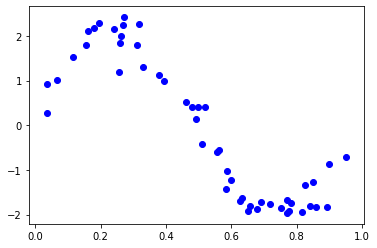
\includegraphics[width=3.4in]{figs/fig1.png}
\end{center}
\caption{Sinusoidal Dataset with added noise}
\label{fig:1}
\end{figure}
The Fig \ref{fig:1} is generated by random values of $x_{n}$ for n =1,2,..,N.
where N=50 in the range [0,1].

The corresponding values of y were generated from the Eq \eqref{eq:1}.The first term $A\sin{2\pi x}$ is computed directly and then random noise samples having a normal(Gaussian) distribution are added inorder to get the corresponding values of y.
\begin{lstlisting}
#Generate the sine curve 
import numpy as np
import matplotlib.pyplot as plt

N = 50
np.random.seed(20)
x = np.sort(np.random.rand(N,1),axis=0)
noise = np.random.normal(0,0.3,size=(N,1))
A = 2.5
y = A*np.sin(2*np.pi*x) + noise

plt.scatter(x,y,c='b',marker='o',label='Data with noise')
plt.xlabel('x');plt.ylabel('y')
\end{lstlisting}
Intialize a regularization parameter $\lambda$ 
\begin{lstlisting}
lamda = 0.00000001522 
poly_deg = 3
\end{lstlisting}
Now, add bias and higher order terms. Here we initialize column 1 with 1 and generate the input matrix as follows
\begin{lstlisting}
F = np.zeros(shape = (N,poly_deg+1))
F[:,0] = 1
for i in range(1,poly_deg+1):
    F[:,i] = np.power(x,i).reshape((N,))    
\end{lstlisting}
The generated matrix would look like
\begin{align}
    \vec{F}= \myvec{ 1 & x_{0} & x_{0}^2 & \ldots & x_{0}^{N-1} \\
		1 & x_{1} & x_{1}^2 & \ldots & x_{1}^{N-1} \\
		1 & x_{2} & x_{2}^2 & \ldots & x_{2}^{N-1} \\
		\vdots & & \vdots &  & \vdots  \\
		    1 & \ldots & \ldots & \ldots & x_{N}^{N-1} }\label{eq:12}
\end{align}
\section{Polynomial Curve Fitting}
The goal is to find the best line that fits into the  pattern of the training data shown in the graph.
We shall fit the data using a polynomial function of the form, 
\begin{align}
     y\brak{w,x}= \sum_{j=0}^{M} w_j x^{j}\\
     y = \hat{\vec{w}}\vec{F}\\
     y = \vec{w}\myvec{ 1 & x_{0} & x_{0}^2 & \ldots & x_{0}^{N-1} \\
		1 & x_{1} & x_{1}^2 & \ldots & x_{1}^{N-1} \\
		1 & x_{2} & x_{2}^2 & \ldots & x_{2}^{N-1} \\
		\vdots & & \vdots &  & \vdots  \\
		    1 & \ldots & \ldots & \ldots & x_{N}^{N-1} }
\end{align}
M is the order of the polynomial
The polynomial coefficient are collectively denoted by the vector $\vec{w}$.The proposed vector $\vec{w}$ of the model referring to Eq \eqref{eq:12} is given by 
\begin{align}
    \hat{\vec{w}} = \brak{\vec{F}^T\vec{F}}^{-1}\vec{F}^Ty \label{eq:13}
\end{align}
%Eq \eqref{eq:13} can be modified by adding a penalty term $\lambda$ to the diagonal %entries of the matrix $F^{T}F$ before taking its inverse given by
%\begin{align}
%     \hat{\vec{w}} = \brak{\vec{F}^T\vec{F} + \lambda I_{M}}^{-1}\vec{F}^Ty %\label{eq:14}
%\end{align}
The values of the coefficients are determined by fitting the polynomial to the
training data.This can be done by minimizing an \textbf{error function} that measures the
misfit between the function y and the training set data points given as
\begin{align}
    \sum_{i=1}^{N}\brak{y_{i} - \sum_{j=0}^{M}x^{j}w_{j}}^2 \label{eq:15}
\end{align}
We add a penalty term at the end to modify the error function Eq \eqref{eq:15}
\begin{align}
    \sum_{i=1}^{N}\brak{y_{i} - \sum_{j=0}^{M}x^{j}w_{j}}^2 + \lambda\sum_{j=0}^{M}w_{j}^2\label{eq:16}
\end{align}
where for some  $t>0$, $\sum_{j=1}^{M}w_{j}^2<t$, 
Eq \eqref{eq:16} can be further expressed as
\begin{align}
    \brak{\vec{y} - \vec{wF}}^T\brak{\vec{y} - \vec{wF}} - \lambda\norm{\vec{w}}^2\label{eq:17}
\end{align}
where $\norm{\vec{w}}^2$ = $\vec{w}^T\vec{w}$.Expand Eq \eqref{eq:17}.
Let 
\begin{align}
    E = \brak{\vec{y} - \vec{wF}}^T\brak{\vec{y} - \vec{wF}} - \lambda\vec{w}^T\vec{w}\\
      = \vec{y}^T\vec{y} - \vec{y}^T\vec{wF} - \vec{w}^T\vec{F}^T\vec{y} + \vec{w}^T\vec{F}^T\vec{F}\vec{w} + \lambda\vec{w}^T\vec{w}\\
      = \vec{y}^T\vec{y} -\vec{w}^T\vec{F}^T\vec{y}  - \vec{w}^T\vec{F}^T\vec{y} + \vec{w}^T\vec{F}^T\vec{F}\vec{w} + \vec{w}^T\lambda\vec{I}\vec{w}\\
      = \vec{y}^T\vec{y} -2\vec{w}^T\vec{F}^T\vec{y}+\vec{w}^T\brak{\vec{F}^T\vec{F} + \lambda\vec{I}}\vec{w}\label{eq:18}
\end{align}
Evaluate $\vec{w}$ that minimizes E. Here, we make use of matrix differentiation rule given as
\begin{align}
    \frac{\partial xA^Tx}{\partial x} = (A + A^T)x = 2Ax
\end{align}
We get 2Ax when A is symmetric. This can be applied here as $\brak{\vec{F}^T\vec{F} + \lambda\vec{I}}$. From Eq \eqref{eq:18}
\begin{align}
    \frac{\partial E}{\partial \vec{w}} = -2\vec{F}^T\vec{y} + 2\brak{\vec{F}^T\vec{F} + \lambda\vec{I}}\vec{w} = 0\\
    \implies \brak{\vec{F}^T\vec{F} + \lambda\vec{I}}\vec{w} = \vec{F}^T\vec{y}\\
    \implies \vec{w} = \brak{\vec{F}^T\vec{F} + \lambda\vec{I}}^{-1}\vec{F}^T\vec{y}
\end{align}
The coefficient $\lambda$ governs the relative importance of the regularization term compared with the sum-of-the-squares term.

First, we take a random guess of the sine curve on the input data
\begin{lstlisting}
plt.plot(np.linspace(0,1,50),np.sin(2*np.linspace(0,1,50)*np.pi),c='g',linewidth=2,label='function generating input data')
\end{lstlisting} 
Form the penalized residual sum of squares as follows
\begin{lstlisting}
W = np.linalg.pinv((F.T.dot(F) + lamda*np.eye(poly_deg+1))).dot(F.T).dot(y)
\end{lstlisting}
Plot the predicted output
\begin{lstlisting}
plt.plot(x,F.dot(W),'r',label='After fitting')
plt.legend()
plt.show()
\end{lstlisting}
You need to vary $\lambda$ to make it work.
\begin{figure}[!h]
\begin{center}
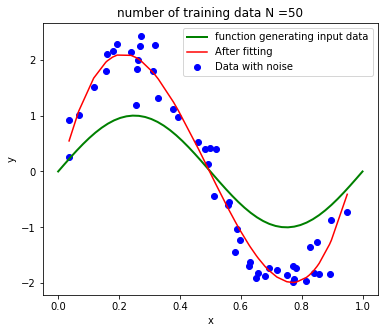
\includegraphics[width=3.4in]{figs/fig2.png}
\end{center}
\caption{Curve Fitting for ln$\lambda = -18$}
\label{fig:2}
\end{figure}
\begin{figure}[!h]
\begin{center}
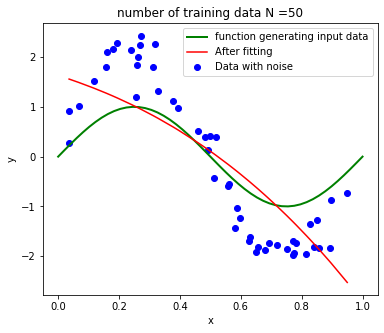
\includegraphics[width=3.4in]{figs/fig3.png}
\end{center}
\caption{Curve Fitting for ln$\lambda = 0$}
\label{fig:3}
\end{figure}
\section{Curve fitting using scikit-learn}
scikit learn is a machine learning python library which features various algorithms and is designed to interoperate with the numpy and scipy libraries.
Here, we import and use linear regression to find the best fit.
\begin{lstlisting}
from sklearn.preprocessing import PolynomialFeatures
sk_poly_deg=3
poly_feature = PolynomialFeatures(degree=sk_poly_deg,include_bias=False)
x_poly = poly_feature.fit_transform(x)

from sklearn.linear_model import LinearRegression
lin_reg=LinearRegression()
lin_reg.fit(x_poly,y)
\end{lstlisting}
\begin{figure}[!h]
\begin{center}
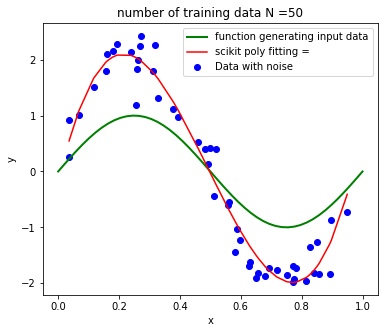
\includegraphics[width=3.4in]{figs/fig4.png}
\end{center}
\caption{Using scikit-learn}
\label{fig:4}
\end{figure}
Python code:
\begin{lstlisting}
https://github.com/Hrithikraj2/EE4015_IDP/blob/main/Assignment3/Assignment_3_Regularization.ipynb
\end{lstlisting}
\end{document}
